\documentclass[border=3pt]{standalone}
% Preâmbulo compartilhado pelos diagramas TikZ da aula 4 de Navegação (Representação de Mapas)
\usepackage[T1]{fontenc}
\usepackage[utf8]{inputenc}
\usepackage{lmodern}
\usepackage{amsmath}
\usepackage{xcolor}
\usepackage{tikz}
\usetikzlibrary{arrows.meta,angles,quotes,decorations.pathmorphing,decorations.pathreplacing,calc,
                positioning,shapes.geometric,shapes.misc,backgrounds,fit,
                math}

% Paleta (mesma dos SVGs originais)
\definecolor{dblue}{HTML}{2A5B8C}
\definecolor{dorange}{HTML}{B3541E}
\definecolor{dgreen}{HTML}{4A7C59}
\definecolor{dred}{HTML}{9C4B4B}
\definecolor{dcream}{HTML}{F4F1EA}
\definecolor{dshade}{HTML}{DDD7C9}

% Função gaussiana (não normalizada por padrão de escala visual)
\pgfmathdeclarefunction{gauss}{3}{%
  \pgfmathparse{1/(#3*sqrt(2*pi))*exp(-((#1-#2)^2)/(2*#3^2))}%
}

% Estilos comuns (prefixo d... para não colidir com chaves internas do pgf)
\tikzset{
  >={Stealth[length=2mm]},
  dguide/.style={gray!55, dashed, line width=0.4pt},
  daxis/.style={gray!60, line width=0.7pt, ->},
  dbody/.style={fill=black!3, draw=black!80, line width=1pt},
  dacc/.style={draw=dblue, line width=1pt},
  dlbl/.style={black!55, font=\small},
  dsub/.style={black!45, font=\footnotesize},
  dstate/.style={circle, draw=black!80, fill=dcream, line width=1pt,
                 minimum size=17mm, font=\large, inner sep=1pt},
  dobs/.style={circle, draw=black!80, fill=dshade, line width=1pt,
               minimum size=14mm, font=\large, inner sep=1pt},
  dbox/.style={rounded corners=2pt, draw=black!80, fill=dcream, line width=1pt,
               align=center, inner sep=6pt},
  dop/.style={circle, draw=black!80, fill=white, line width=1pt,
              minimum size=6mm, inner sep=0pt, font=\small},
  dtrans/.style={->, dblue, line width=1pt},
  dmeas/.style={->, dorange, line width=1pt},
  dcurve/.style={line width=1pt, dblue},
  dcurveb/.style={line width=1.4pt, dorange},
}

\begin{document}
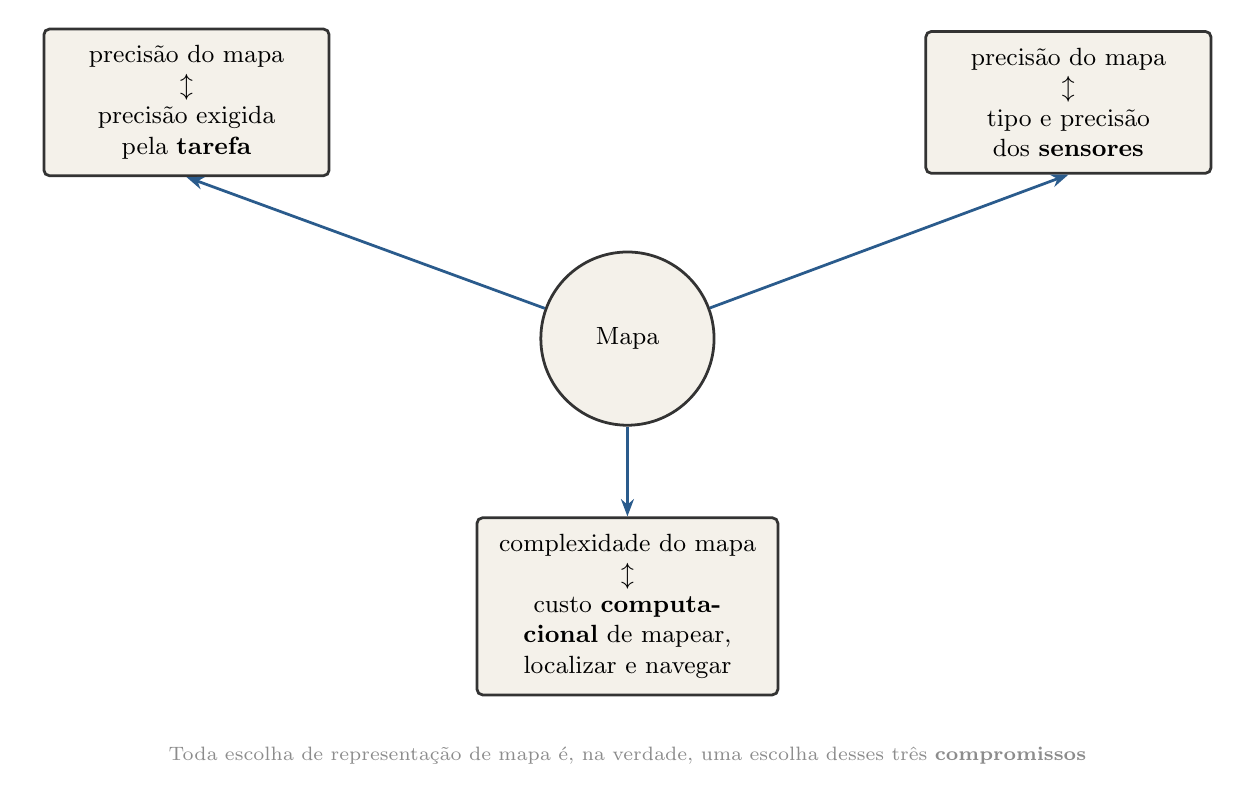
\begin{tikzpicture}[x=1cm,y=1cm]

  \node[dstate, minimum size=22mm, font=\small, align=center] (m) at (0,0) {Mapa};

  \node[dbox, text width=3.2cm, font=\small] (a) at (-5.6,3.0) {precisão do mapa\\ $\updownarrow$\\ precisão exigida pela \textbf{tarefa}};
  \node[dbox, text width=3.2cm, font=\small] (b) at (5.6,3.0) {precisão do mapa\\ $\updownarrow$\\ tipo e precisão dos \textbf{sensores}};
  \node[dbox, text width=3.4cm, font=\small] (c) at (0,-3.4) {complexidade do mapa\\ $\updownarrow$\\ custo \textbf{computacional} de mapear, localizar e navegar};

  \draw[dtrans, -{Stealth[length=2.2mm]}] (m) -- (a.south);
  \draw[dtrans, -{Stealth[length=2.2mm]}] (m) -- (b.south);
  \draw[dtrans, -{Stealth[length=2.2mm]}] (m) -- (c.north);

  \node[dsub, font=\scriptsize, align=center, text width=15cm] at (0,-5.3)
     {Toda escolha de representação de mapa é, na verdade, uma escolha desses três \textbf{compromissos}};

\end{tikzpicture}
\end{document}
